\clearpage
\chapter{ПРАКТИЧЕСКАЯ ЧАСТЬ}

Вышеописанные исследования привели к чётко поставленной задаче --- реализовать программно-аппаратный комплекс, который позволял бы максимально доступным образом создавать диалоговых когнитивных роботов. Программная часть должна реализовывать логику робота, используя реактивно"=делиберативный подход. Аппаратная часть комплекса должна быть основана на микроконтроллерах Arduino и микрокомпьютерах Raspberry Pi. В разделе \ref{apparat-platform} была поставлена задача реализовать взаимодействие двух устройств: Arduino и Raspberry Pi. Было принято решение основать взаимодействие устройств на обмене командами из множества определяемых пользователем команд.

\section{Основные этапы в разработке решения задачи, сформулированной в ВКР}
Основными этапами разработки явились:
\begin{enumerate}
\item подготовка аппаратной платформы решения 
\begin{itemize}
    \item исследование микроконтроллеров Arduino и микрокомпьютеров Raspberry Pi, представляющих основу аппаратной части, с точки зрения программиста
    \item разработка единой аппаратной платформы, объединяющей Arduino и Raspberry Pi в единый элемент, реализующий поставленную задачу
\end{itemize}

\item разработка необходимого программного обеспечения
\begin{itemize}
    \item выбор технологий для построения программного решения поставленной задачи
    \item выделение ключевых подзадач поставленной задачи в самостоятельные единицы, подлежащие разработке
    \item разработка выделенных на предыдущем этапе элементов
\end{itemize}

\item отладка разработанного решения

\item доработка решения с учётом требований потенциальных пользователей
\begin{itemize}
    \item анализ разработанного решения потенциальными пользователями
    \item доработка разработанного решения с учётом требований потенциальных пользователей
\end{itemize}

\item применение разработанного решения к реальной задаче  
\begin{itemize}
    \item реализация пробного проекта вместе с потенциальными пользователями решения
    \item получение обратной связи от потенциальных пользователей разработанного решения и сторонних компетентных специалистов
\end{itemize}

\item публикация законченного разработанного решения как готового
\begin{itemize}
    \item внедрение разработанного решения в технологический стек потенциальных пользователей решения
    \item публикация исходного кода разработанного решения
\end{itemize}
\end{enumerate}

\noindent 
Этапы разработки подробно раскрыты ниже.

\section{Подготовка аппаратной платформы решения}
\subsection{Выбор технологии, связывающей Arduino и Raspberry Pi}
В разделе \ref{apparat-platform} были рассмотрены средства ввода"=вывода доступные как на устройствах Arduino, так и на устройствах Raspberry Pi.
Хотя оба класса устройств способны использовать три технологии ввода"=вывода (пины), выбранная в качестве используемой технология (пины) не явилась спорным решением.

Взаимодействие Arduino и Raspberry Pi на низком уровне запланировано быть реализованым не конечным пользователем решения, а разработчиками решения. Это мотивирует постараться выбрать максимально гибкое решение, которое было бы легко перенастраивать на самом низком уровне, если этого потребует процесс разработки --- разработчик, в отличие от конечного пользователя, готов исследовать сложную технологию для решения какой-то проблемы. 

Технологии ethernet и usb позволяют обмениваться большими объёмами данных и часто предоставляют программисту удобный высокоуровневый интерфейс для этого. Так как в поставленой задаче было принято решение организовать взаимодействие между Arduino и Raspberry Pi на основе некоторого множества определяемых команд, способность передавать большие объёмы данных между устройствами оказалась излишней. пины же, предоставляющие простейший низкоуровневый способ обмена информацией побитно, прекрасно подошли для задачи.

Мощность множества команд взаимодействия Arduino и Raspberry Pi ограничивается сверху количеством пины.

Получившаяся в результате аппаратная платформа (представлена на рис. \ref{apparat_plfm_img}) выглядит следующим образом: микроконтроллер Arduino и микрокомпьютер Raspberry Pi, общающиеся через пины.

\begin{figure}[H]
    \centering
    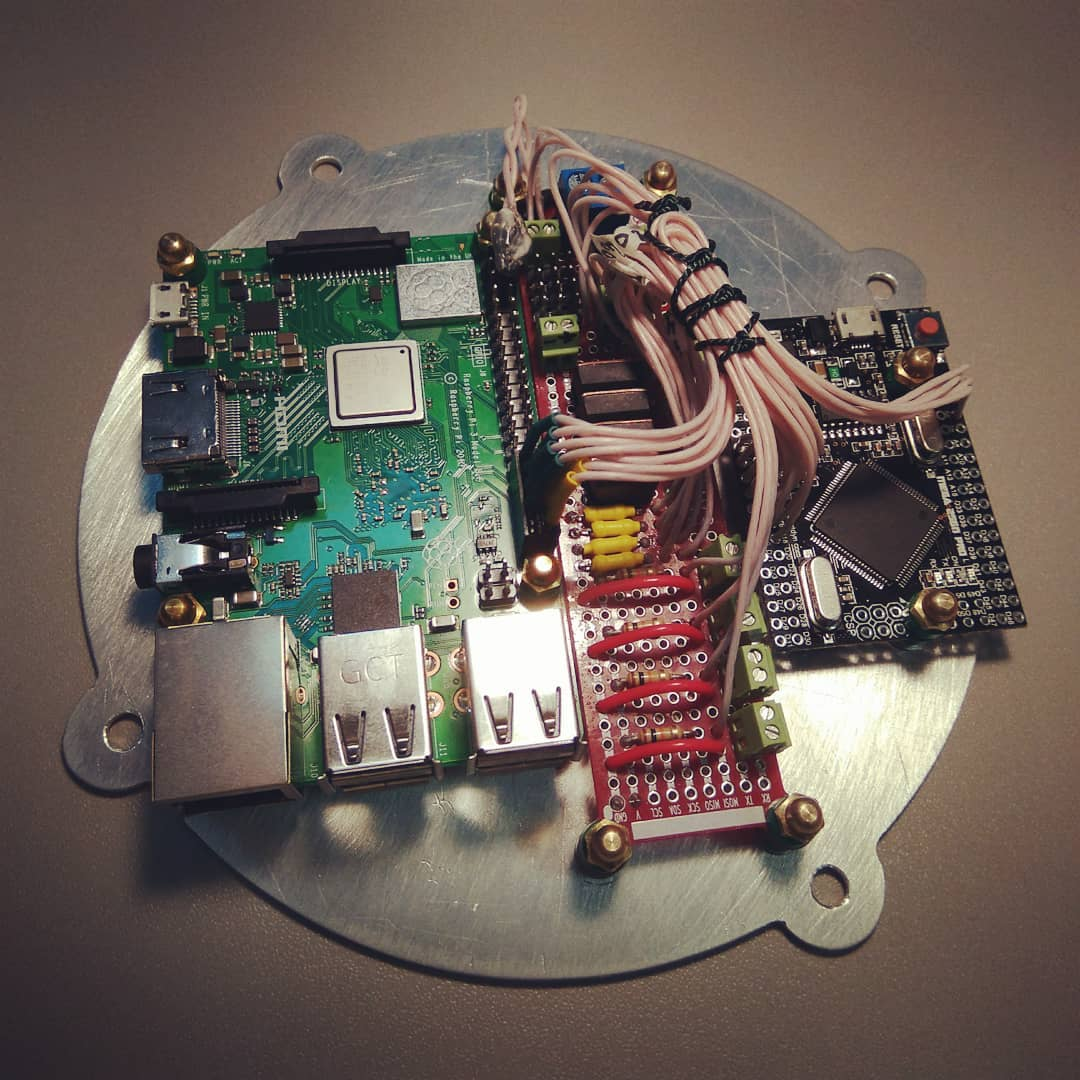
\includegraphics[scale=0.4]{images/apparat_platform.jpg}
    \caption{Реализация аппаратной платформы}
    \label{apparat_plfm_img}
\end{figure}

\section{Разработка необходимого программного обеспечения}

Схема разработанного программного обеспечения представлена на рис. \ref{PO_scheme_img}.

\begin{figure}[H]
    \centering
    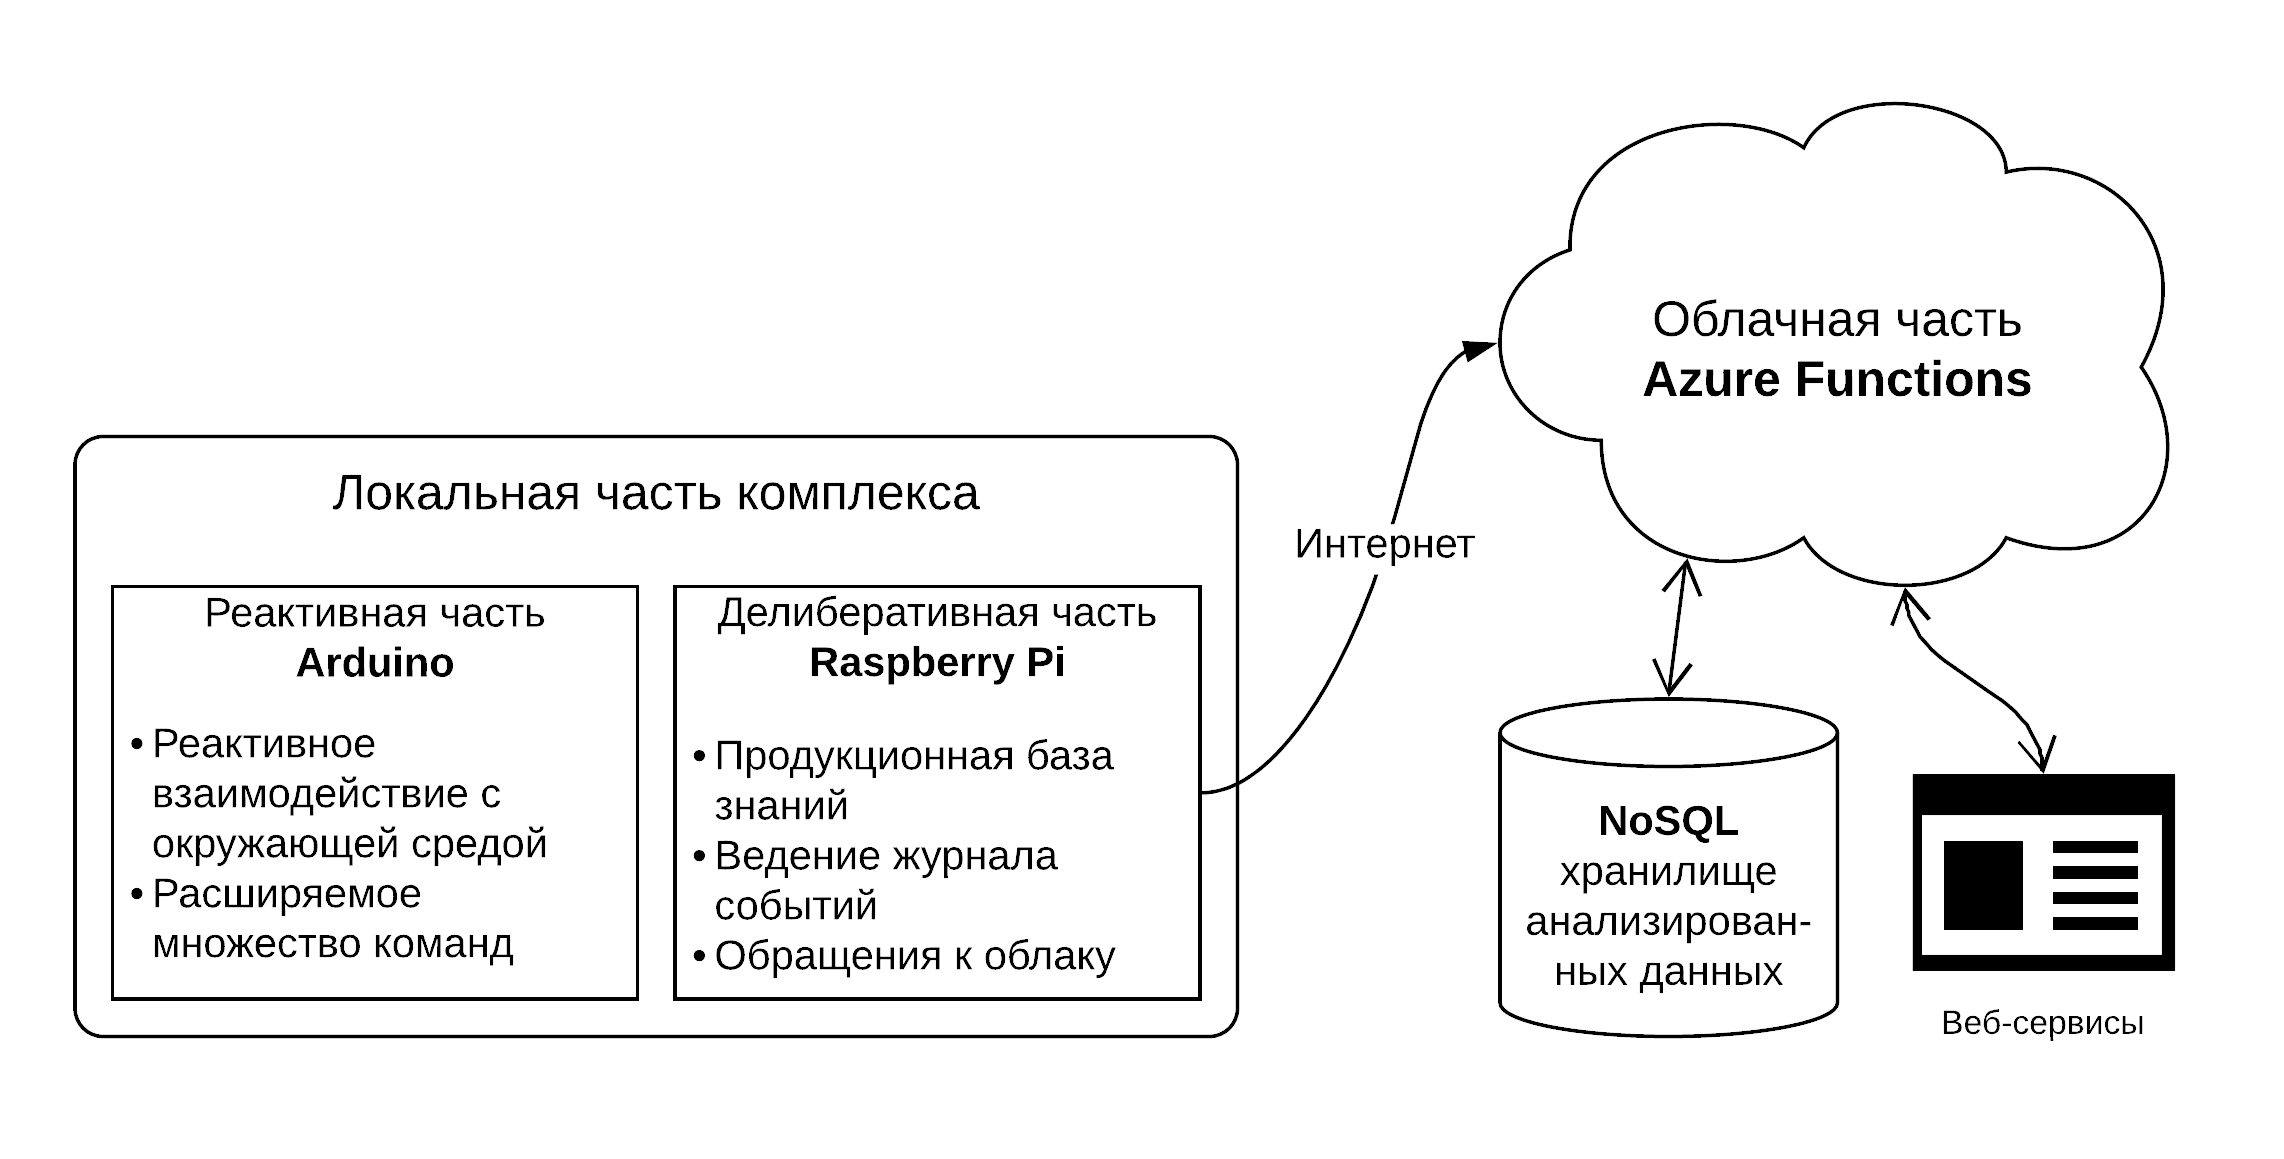
\includegraphics[scale=0.2]{images/po.png}
    \caption{Прораммная архитектура решения}
    \label{PO_scheme_img}
\end{figure}

\subsection{Разделение задач между Arduino и Raspberry Pi}
Задачи, возникающие в процессе работы, были разделены между микроконтроллером Arduino и микрокомпьютером Raspberry Pi следующим образом: 
\begin{itemize}
    \item Rasbperry Pi \begin{itemize}
        \item реализует делиберативную составляющую диалога
        \item предоставляет интерфейс для реализации условий, проверяемых в процессе логического вывода
        \item принимает решения о выполнении тех или иных действий, требуемых текущим состоянием диалога
        \item предоставляет программный интерфейс для реализации подзадач общения с собеседником на стороне Raspberry Pi
    \end{itemize}
    
    \item Arduino \begin{itemize}
        \item реализует реактивную составляющую диалога
        \item предоставляет Raspberry Pi интерфейс для реализации подзадач общения с собеседником на стороне Arduino
    \end{itemize}
\end{itemize}

\subsection{Выбор ключевых элементов программного обеспечения}
\subsubsection{Ключевые элементы программного обеспечения Arduino}
Arduino не предоставляет какого-то выбора опорных элементов для программных решений: программисту доступна лишь возможность заливать код, написанный на Си"=подобном языке, на плату. 

\subsubsection{Выбор операционной системы для Raspberry Pi}
Семейство микрокомпьютеров Raspberry Pi может работать под управлением операционных систем, которые можно разбить на два класса: Unix"=подобные и Windows.

Исследование относительного объёма доступных информационных материалов по Arduino и Raspberry Pi показало, что несмотря на меньшую свободу действий, представляемую Windows, количество информации о разработке под Raspberry Pi, управляемую операционной системой Windows на порядок превосходит количество информации о разрабоке под Raspberry Pi, управляемую операционной системой *nix. 

\subsubsection{Архитектура разработанного программного обеспечения на стороне Raspberry Pi}
Программное обеспечение было реализовано в формате UWP"=приложения --- де"=факто стандартном формате для приложений под Windows IoT.

Когнитивные функции приложения были вынесены в облако чтобы разгрузить вычислительно слабый Raspberry Pi.

Локальная часть программного обеспечения в свою очередь состоит из нескольких фундаментальных частей, описанных ниже.

\paragraph*{Описание облачной части решения.} В облако были вынесены когнитивные функции, получение обновлений и сбор всевозможной информации о работе приложения --- как сбор информации о данных, подвергающихся когнитивному анализу, так и сбор логов.

Сбор логов и публикация обновлений через интернет дают возможность отслеживать поведение программы и исправлять какие-то ошибки, не находясь рядом с роботом, построенным на платформе, разработанной в рамках выпускной работы.

Сбор всевозможных анализируемых данных, а также использование лог"=записей, позволяют исследовать типовые случаи, в которые попадает робот, что позволяет обновлять программное обеспечение и максимизировать качество решения поставленной задачи.

\paragraph*{Описание локальной части решения.} Локальная часть состоит из двух частей. С точки зрения логики решаемой задачи основной частью является часть, реализующая делиберативный подход --- она представлена как исполнитель системы, основанной на множестве правил. Другая же часть отвечает за использование ресурсов, предоставляет системе из правил доступ к медийным возможностям Raspberry Pi, осуществляет координацию параллельно работающих многопоточных элементов логики, осуществляет обработку ошибок.
В отдельный компонент, не имеющий ценности с точки зрения постановки задачи, но очень ценный на практике при исследовании поведения полученной системы, выделено средство логирования, отвечающее за журналирование всех событий, происходящих в системе.

Подробнее о системе, основанной на правилах: для удобного написания правил был написан язык, подобный прологу. Правила реализованы как пары $<\texttt{условие},\  \texttt{действие}>$. Классы условий и действий представлены диаграммах на рис. \ref{action_diag_ing},  рис. \ref{expression_diag_ing}.

\begin{figure}[H]
    \centering
    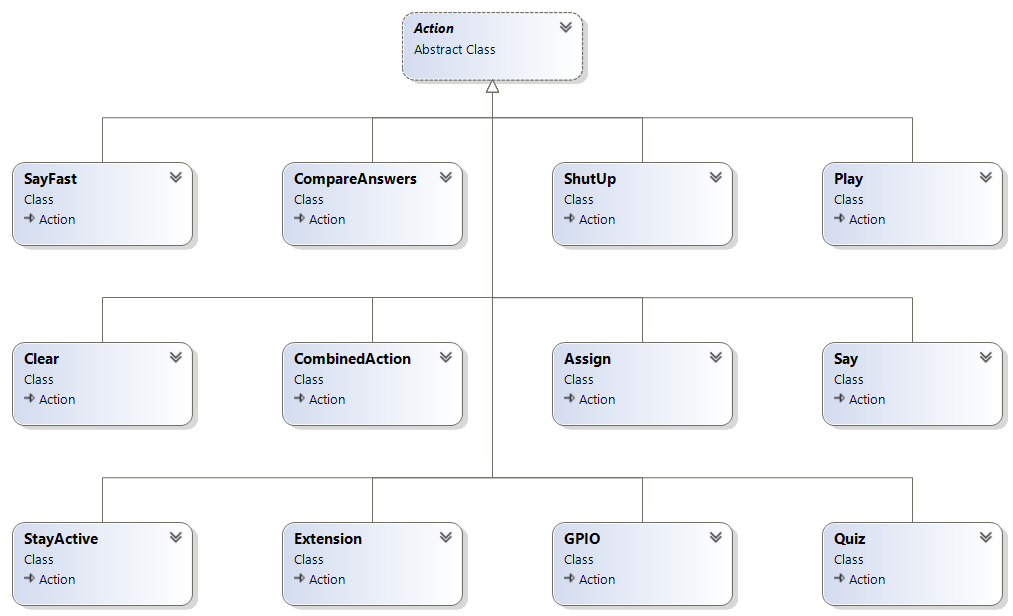
\includegraphics[scale=0.75]{images/action.png}
    \caption{Диаграмма классов действий}
    \label{action_diag_ing}
\end{figure}

\begin{figure}[H]
    \centering
    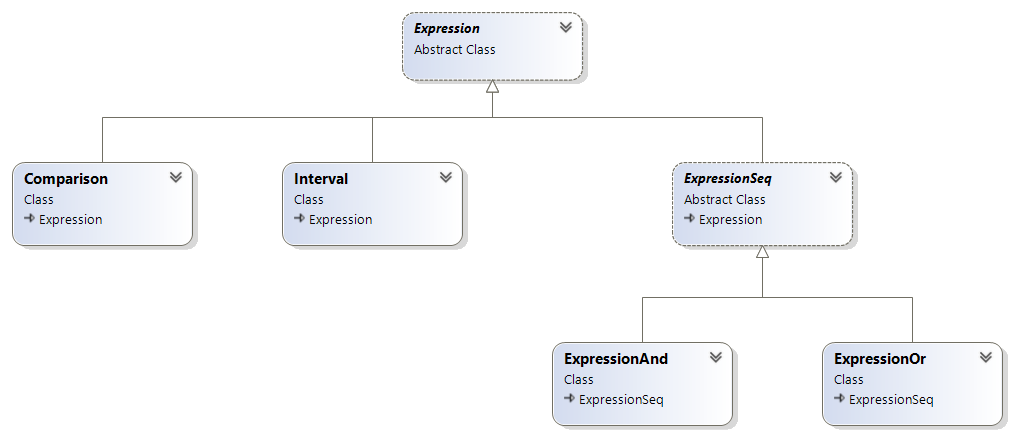
\includegraphics[scale=0.75]{images/expression.png}
    \caption{Диаграмма классов условий}
    \label{expression_diag_ing}
\end{figure}

\section{Доработка решения с учётом требований потенциальных пользователей}
Полученная система была представлена компании МеханиУм и было принято решение о разработке прототипа робота, управляемого системой. Были выдвинуты требования, необходимые для решения задачи, основным требованием стала необходимость воплотить принятое решение об использовании компьютерного зрения в качестве источника информации, подлежащей когнитивному анализу.

В систему был добавлен механизм обнаружения лиц, появляющихся перед роботом, оперативное получение информации о количестве лиц, находящихся перед роботом, были произведены необходимые мелкие доработки, позволяющие использовать информацию, полученную в результате и в процессе анализа лиц, в базе знаний робота.

В процессе добавления механизма анализа лиц стало очевидно, что в будущем при расширении функционала решения аналогичным образом необходимо иметь удобный шаблон для добавления нового функционала. Был произведён глубокий рефакторинг кода, выделивший единое место и структуру для добавления логики, расширяющей функционал решения.


\section{Применение разработанного решения к реальной задаче}
На основе разработанного решения был построен робот <<Подушка --- помощник космонавта Лариса Сергеевна>>. Робот явился тематическим когнитивным диалоговым роботом, способным как решать задачи обучения и общения --- вести беседу, проводить тестирования ---, так и задачи развлекательные --- например, исполнение танцев.


\section{Публикация законченного разработанного решения как готового}
Разработка решения велась с использованием системы контроля версий Git, а именно --- GitHub. Сначала, будучи проектом, зародившимся в Microsoft Evangelism, разработка велась в репозитории Microsoft Evangelism Russia, позже, в процессе совместной с командой МеханиУм работы над решением, в качестве основного репозитория стал использоваться репозиторий команды МеханиУм, релизы основной ветки которого переносятся в репозиторий Microsoft Evangelism Russia.

\section{Части программы, подлежащие оптимизации}
Ключевым местом в логике всего разработанного решения является движок базы знаний. На момент защиты выпускной квалификационной работы движок базы знаний основан на максимально наивных алгоритмах, которые, несмотря на преимущество, состоящее в простоте понимания бесхитростных решений, могут быть оптимизированы в случае появления необходимости в этом.

Оптимизации подлежит алгоритм, отвечающий за парсинг текста базы знаний -- сейчас используется наивный, жадный и вычислительно дорогой подход, основанный на регулярных выражениях.

Оптимизации подлежит также алгоритм выбора правил, подлежащих исполнению --- сейчас используется наивный подход, проверяющий условия выполнения всех правил, а оптимальный подход использовал бы идею о том, что база знаний может быть рассмотрена как граф.